\section{Konvolucijske neuronske mreže}

Konvolucijske neuronske mreže razvile su se početkom ovog tisućljeća \citep{ObjectRecognition}. One su prilagođene za tipove podataka s topologijom rešetke (1D - vremenski slijed, 2D - slika/video). Standardna struktura konvolucijskog modela prikazana je na slici \ref{img:cnn}.

\begin{figure}[htb]
\centering
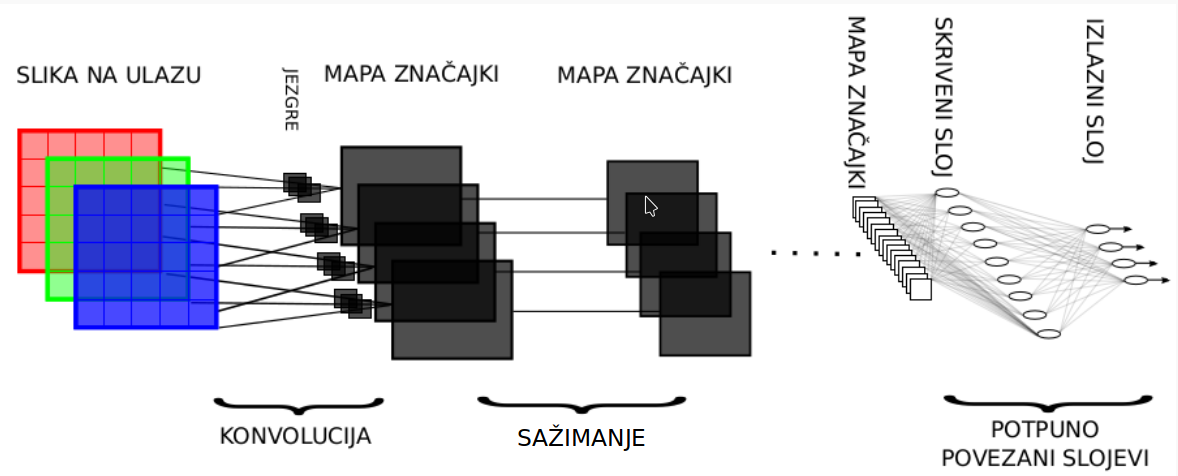
\includegraphics[width=12cm]{img/CNN.png}
\caption{Klasična struktura konvolucijske neuronske mreže \citep{duPredavanja}}
\label{img:cnn}
\end{figure}

Konvolucijske neuronske mreže dobile su ime po matematičkoj operaciji koja se naziva \textbf{konvolucija}. Konvolucija je matematički operator koji od dvije funkcije $x$ i $w$ prizvodi treću, $h$, koja predstavlja količinu preklapanja između funkcije $x$ i okrenute i prevedene verzije funkcije $w$. Tu operaciju možemo zapisati kao:

\begin{equation}
h(t) = \int_{-\infty}^{\infty} x(\tau)w(t - \tau)d\tau
\label{eq:conv_1}
\end{equation}
što se još zapisuje kao:

\begin{equation}
h(t) = (x * w)(t)
\label{eq:conv_2}
\end{equation}
gdje su:

\begin{itemize}
\item funkcija $x$ - ulaz
\item funkcija $w$ - jezgra
\item funkcija $h$ - \textbf{mapa značajki}, rezultat konvolucije
\end{itemize}

\begin{figure}[htb]
\centering
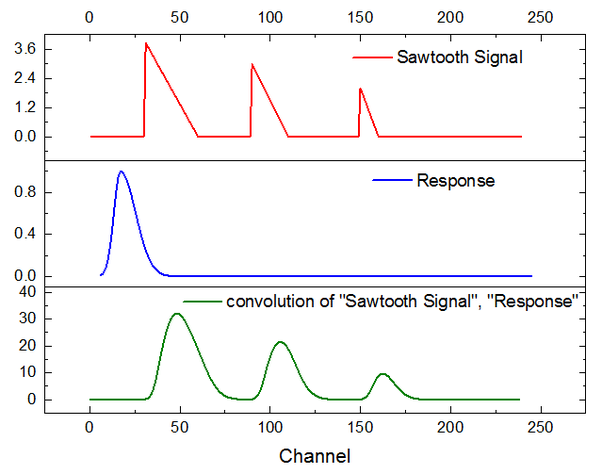
\includegraphics[width=10cm]{img/MathConvolution.png}
\caption{Konvolucija dviju funkcija}
\label{img:convolution}
\end{figure}

U primjenama su $x$ i $w$ obično višedimoenzionalne funkcije, $\mathbf{x}(t), \mathbf{w}(t) \in \mathbb{R}^d$. Konvolucija se može primjenjivati i više dimenzija, npr. slika (dvondimenzionalan i diskretan ulaz), tada konvolucija izgleda kao što je prikazano jednadžbom \ref{eq:2d_conv}.

\begin{equation}
h(i,j) = (\mathbf{X} * \mathbf{W})(i,j) = \sum_{m_{min}}^{m_{max}} \sum_{n_{min}}^{n_{max}} \mathbf{X}(m,n)\mathbf{W}(i - m, j - n)
\label{eq:2d_conv}
\end{equation}

\begin{figure}[htb]
	\centering
	\begin{subfigure}[b]{0.8\linewidth}
		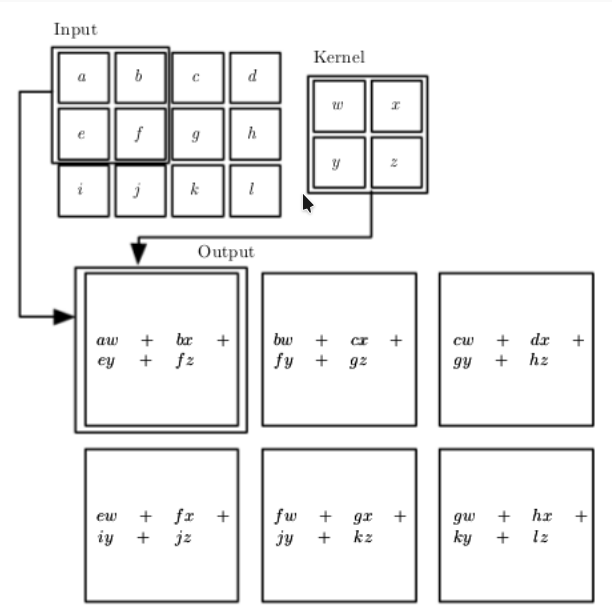
\includegraphics[width=\linewidth]{img/ConvExample.png}
		\caption{Računanje mape značajki sa slike \citep{duPredavanja}}
		\label{img:feature_map1}
	\end{subfigure}
	\begin{subfigure}[b]{0.8\linewidth}
		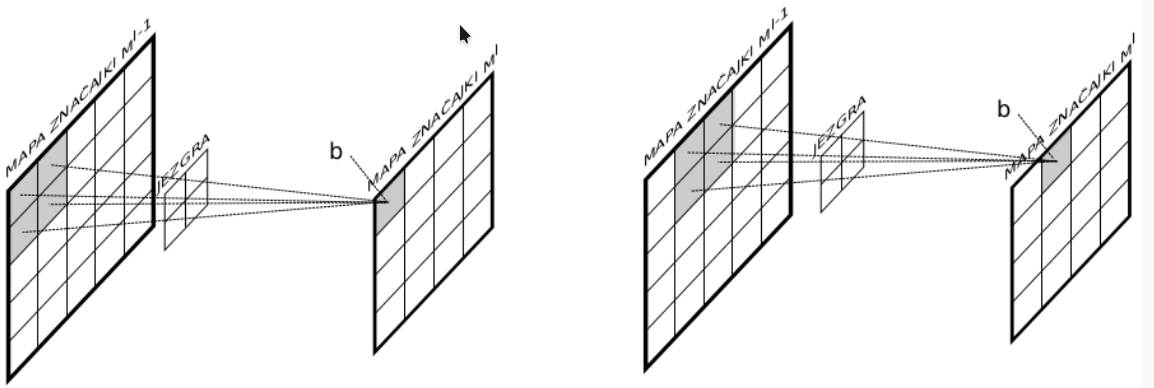
\includegraphics[width=\linewidth]{img/ConvExample2.png}
		\caption{Računanje mape značajki iz druge mape značajki \citep{duPredavanja}}
		\label{img:feature_map2}
	\end{subfigure}
	\caption{Računanje mapa značajki}
	\label{img:feature_map}
\end{figure}

Slika \ref{img:feature_map}.\subref{img:feature_map1} prikazuje kako jezgra (\textit{engl. kernel}) "klizi" po slici i računa pojedini element mape značajki. Slika \ref{img:feature_map}.\subref{img:feature_map2} prikazuje računanje mape značajki iz druge mape značajki. Na ovoj slici vidljivo je da elementi izlazne mape značajki ovise o lokalnom susjedstvu (čija veličina ovisi o veličini jezgre) elemenata ulazne mape značajki. Važno je napomenuti da se na obje slike svi elementi mape značajki računaju uz pomoć istog skupa parametara. 
Kod konvolucije, važno je napomenuti da modelira samo lokalne interakcije (ponovno, ovisno o veličini jezgre) te da dijeli parametre. Dijeljenje parametara, prikazano na slici \ref{img:param_sharing}, važno je svojstvo konvolucijskih neuronskih mreža jer im omogućuje ekvivarijantnost obzirom na pomak. Takvo dijeljenje težina omogučava da mreža nauči relevantne i diskriminativne značajke. Jezgre se specijaliziraju za određenu funkciju, primjerice detekcija horizontalnih i vertikalnih bridova, odziv na različite uzorke i slično. Time postaju slične npr. Haarovim i drugim značajkama. Bez dijeljenja težina dijelovi neuronske mreže bili bi pretrenirani na određeni detalj podataka. Kod potpuno povezanog sloja svaki izlaz je povezan sa svim ulazima, a kod konvolucije samo sa malim dijelom ulaza što jako smanjuje i broj parametara koje je potrebno naučiti te omogućuje bržu evaluaciju. To dakle znači i manje podataka potrebno za trening da bi se postigla jednaka točnost modela, a istovremeno smanjuje opasnost pretreniranja modela. Problemi za konvoluciju nastaju kod transformacija ulaza koje nisu translacijske, na primjer, rotacija i skaliranje.

\begin{figure}[htb]
\centering
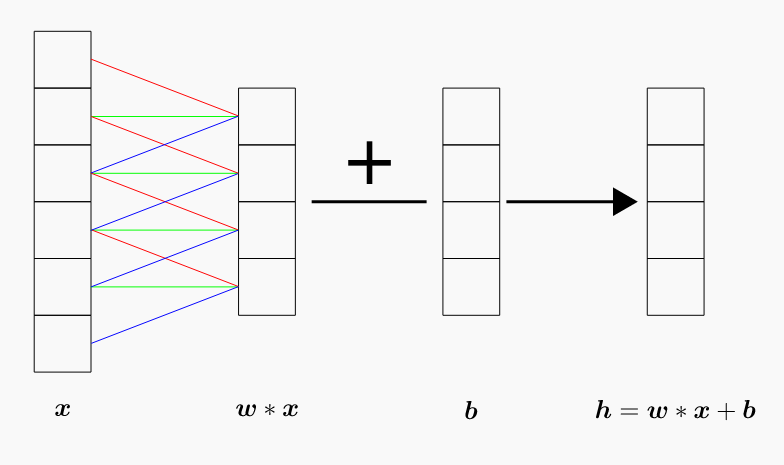
\includegraphics[width=10cm]{img/ParameterSharing.png}
\caption{Dijeljenje parametara. Plava, crvena i zelena crta predstavljaju parametre jezgre koji klize po ulaznom nizu i stvaraju mapu značajki $w * x$ \citep{duPredavanja}}
\label{img:param_sharing}
\end{figure}

\par \bigbreak
\textbf{Sloj sažimanja} (\textit{engl. pooling layer}) ima zadaću mapirati skup prostorno bliskih značajki na ulazu u jednu značajku na izlazu. Obično se za funkciju sažimanja uzima neki statistički pokazatelj ulaznih značajki kao što su srednja ili maksimalna vrijednost. Ovim postupkom dodatno se povećava invarijantnost na pomak. Invarijantnost na pomak je vrlo korisna ako pretpostavljamo da je za raspoznavanje bitnije detektirati prisutnost određene značajke, nego njezinu točnu lokaciju. Veličina regije sažimanja regulira dozu invarijantnosti: što je regija sažimanja veća, to je mreža invarijantija na veće pomake. Sažimanje se može obaviti ne samo preko susjednih značajki u istoj mapi, nego i preko različitih mapa: tada mreža može naučiti invarijantnost i na druge transformacije. Slika \ref{img:pooling} prikazuje sažimanje maksimalnom vrijednosti (\textit{engl. max-pooling}). 

\begin{figure}[htb]
\centering
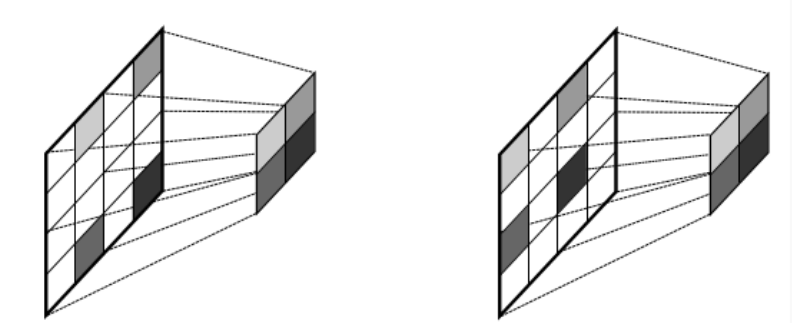
\includegraphics[width=10cm]{img/Pooling.png}
\caption{Max-pooling \citep{duPredavanja}}
\label{img:pooling}
\end{figure}
Sažimanje kao posljedicu ima sažimanje mape značakji $k$ puta, gdje je $k$ veličina regije koja se sažima. Sažimanje je izuzetno korisno i zbog toga što omogućava procesiranje ulaza (npr. slika) različitih veličina. 

Korištenjem konvolucijskog sloja i sloja sažimanja, u model se ugrađuju određene pretpostavke. Pretpostavke uvedene konvolucijom su:
\begin{itemize}
\item pretpostavljamo topologiju podataka
\item predikcija je kovarijantna s pomakom
\end{itemize}
Pretpostavka uvedena slojem sažimanja jest da je predikcija invarijantna na male pomake. Ove pretpostavke povećavaju pristranost i smanjuju varijancu. U teoriji, to dovodi do podnaučenosti mreže te time i bolje generalizacije. No, u praksi nema podanučenosti, ali pokazalo se da konvolucijski modeli generaliziraju bolje od potpuno povezanih slojeva. Konvolucijski slojevi mogu se zamisliti kao specijalni slučaj potpuno povezanih slojeva u kojima su sve težine koje nisu unutar područja jezgre postavljene na nulu. 

Slika \ref{img:cnn} prikazuje klasičnu strukturu konvolucijske neuronske mreže.  Na ulazu može biti jedna monokromatska slika ili višekanalna slika u boji. Zatim slijede naizmjenice konvolucijski slojevi i slojevi sažimanja.  Na samom kraju nalazi se nekoliko potpuno povezanih slojeva (perceptron) koji su jednodimenzionalni, uključujući i izlazni sloj.


